The testing implementation was developed with high modularity in mind,
since it is meant to be a proof-of-concept implementation and not a
production grade system. High modularity also makes development easier
and the system more robust against changes, two very important
qualities during this project.

The implementation is written in Python and consists of three main parts:
\begin{description}
  \item[Particle Filter] A direct  implementation of the procedure in
    table \ref{alg:pf}.
  \item[Database] A database with functions for extracting transition
    hypotheses. Provides the prediction PDF $\cprobnext{x}$ to the
    particle filter.
  \item[Tracker] Manages the model and performs matching between
    hypotheses and images. Provides the filtering PDF
    $\cprob{I_n}{x_n}$ to the particle filter.
\end{description}

\section{The particle filter}
The particle filter implementation is a direct implementation of the
procedure in table \ref{alg:pf}. It is implemented as a function that
takes the parameters $X_{t-1}$, $I_t$, \texttt{importance\_function} and
\texttt{sampling\_function}. The parameters are the hypotheses from
the last time step, the current video frame and the functions to use
as \textsc{Predict} and \textsc{Importance} in \ref{alg:pf},
respectively. This means that the particle filter function is general
and independent of the model used. The implementations of
\textsc{Predict} and \textsc{Importance} are provided by the database
and tracker, respectively.

\subsection{Initilization $x_0$}
The test implementation needs to be manually initialized. When
tracking generated whiskers, the states were always known and program
could therefore be programmatically inserted. When testing on real
whiskers, the start states were calculated by manually selecting five
or six pixels along each whisker and using a MATLAB script to find the
least squares solution for the coefficients $\langle a_1, a_2, a_3
\rangle$. The problem of automatic initialization is a difficult one
\cite{Hedvig}, and is not covered in this thesis.

\section{The state transition database}

\subsection{Data format}
A \emph{state transition} is a pair $\trans$ that denotes we have
observed a system go from state $\tf$ to state $\tt$ in one time
step. Technically, the state transition database is implemented as an
SQLite3 database. One transition is represented in the database as a
row with the state parameters of the model before and after the
transition. The set of transitions in the database will be denoted \TS.

\subsection{Prediction $\cprobnext{x}$}

\begin{table}[h]
  \begin{codebox}
    \Procname{$\proc{DB-Predict} (x_{t-1})$}
    \li $ x_t \gets 0$
    \li $ W \gets 0$
    \li \ForEach $(\tf, \tt) \in \TS$
    \li \Do
      \li $ w \gets \left(\Lpnorm[p]{\tf - x_t}\right)^{-a}$
      \li $ x_t \gets x_t + w \cdot \tt$
      \li $ W \gets W + w$
    \End
    \li Take $v \sim \ndist{0}{\Sigma}$
    \li \Return $ x_t / W + v $
  \end{codebox}
  \caption{Pseudocode for the prediction function, with the parameters $a$ and $p$.}
  \label{alg:predict}
\end{table}

The \textsc{Predict} function in table \ref{alg:pf} is implemented as
a weighted mean of the state transitions in the database. The function
is stated in table \ref{alg:predict}. Notice the parameters $a$ and
$p$. $p$ is a positive integer that determines which $\Lp$ space to
compute the norm in. $a$ is a positive number, and determines how fast
the weight $w$ declines with the distance $\Lpnorm[p]{\tf -
  x_{t-1}}$. A high $a$ means closer transitions get a much higher
weight than ones far away, see figure \ref{fig:x-to-the-minus-a}.

At this point, however, the prediction is still deterministic - the
result for any given input $x_{t-1}$ is completely determined by the
parameters $a$ and $p$ and the content of the database. A
deterministic prediction function is not desirable, since the
filtering step only removes improbable hypotheses and replaces them
with duplicates of probable ones. This means that having a
deterministic prediction effectively reduces the number of hypotheses
with each filtering step. For this reason, the result is offset by a
small normal distributed term\footnote{The offset $v$ is a polynomial
  $\Spline[b]{\omega}$ where coefficient $b_i \sim \ndist{0}{\sigma_i}
  $ and $\sigma_i$ is different for the different $i$.} $v$ to make
the prediction nondeterministic.

\begin{figure}[ht]
  \centering
  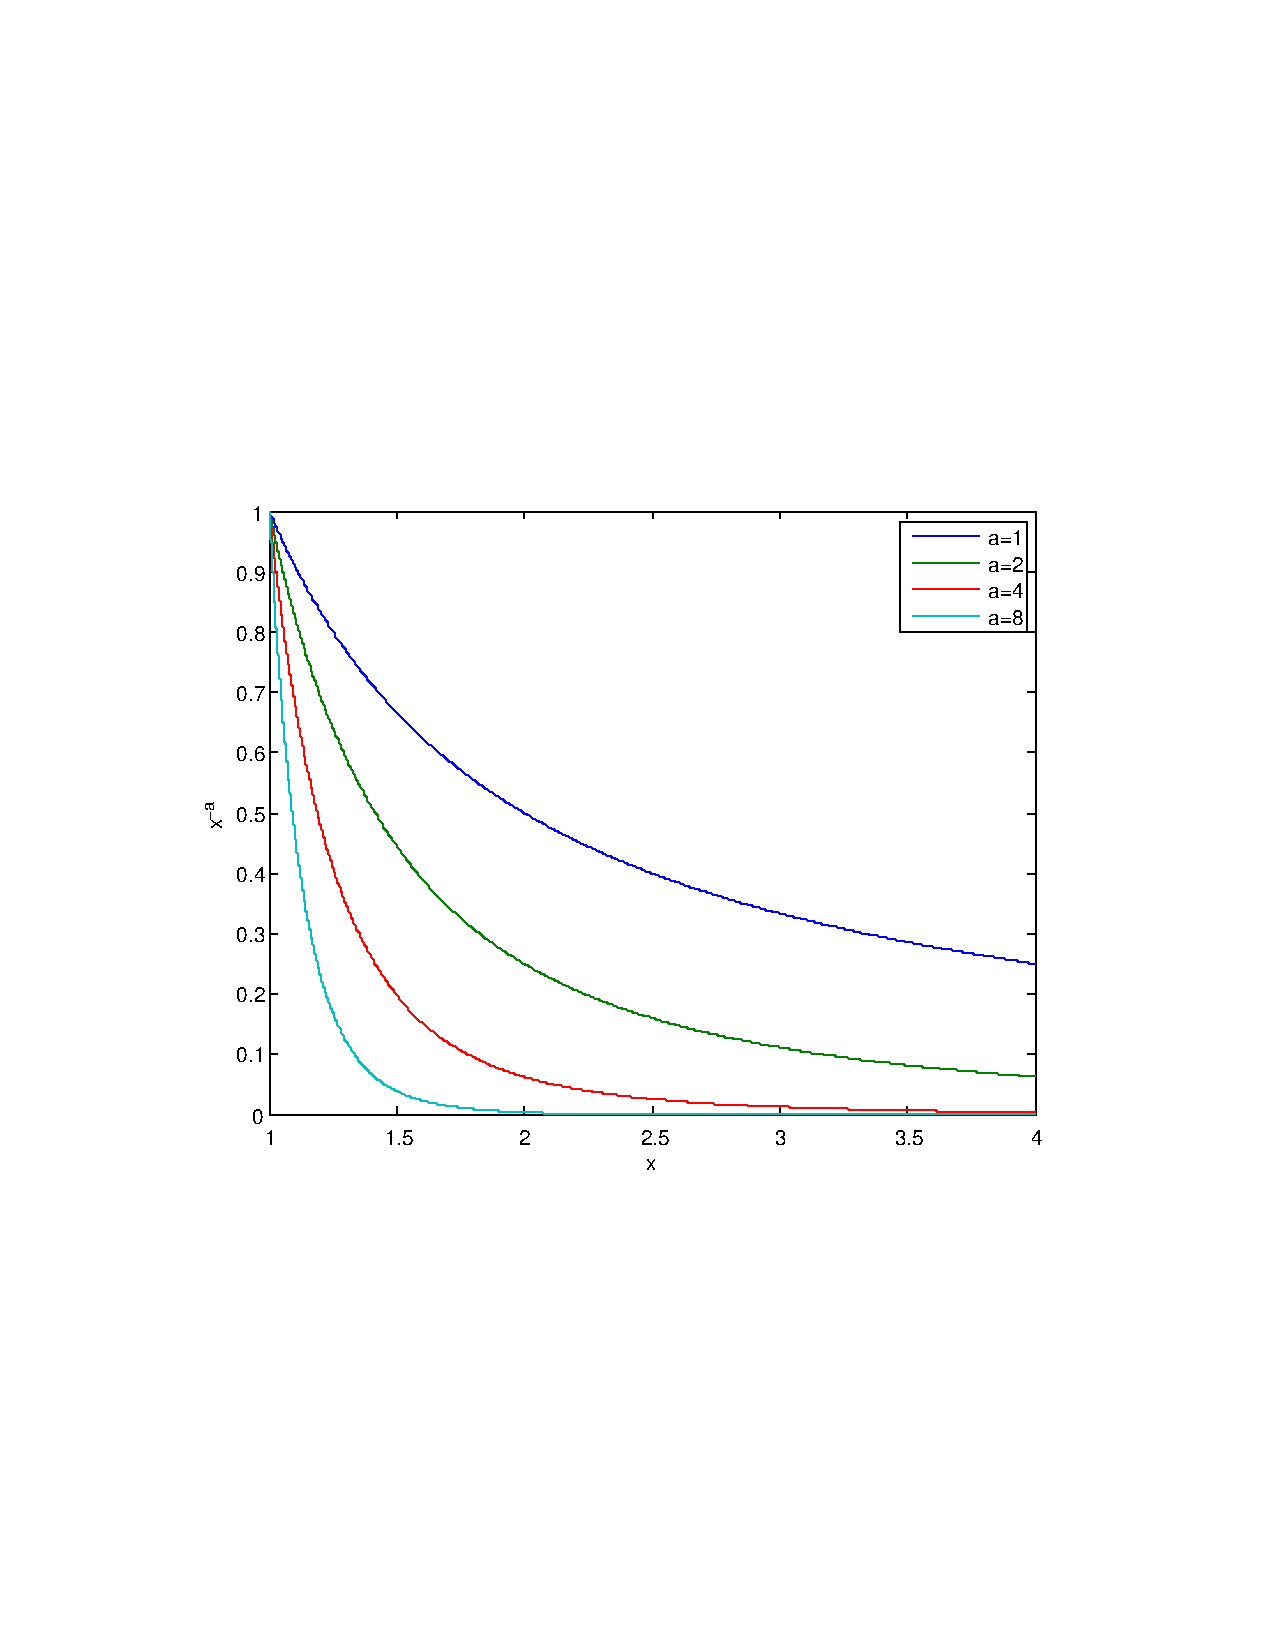
\includegraphics[width=0.4\textwidth,trim=65mm 65mm 65mm 65mm]{x-to-the-minus-a.pdf}
  \caption{Transitions closer to $x_{t-1}$ recieve a much greater
    weight if $a$ is large.}
  \label{fig:x-to-the-minus-a}
\end{figure}

\section{Tracker}

The tracker uses the whisker model described in chapter 4 and
internally represents whiskers with the tuple $\coeffs$ of polynomial
coefficients.

\subsection{Filtering $\cprob{I_t}{x_t}$}
\label{sec:filtering}

\begin{table}[h]
  \begin{codebox}
    \Procname{$\proc{Importance} (x_t, I_t)$}
    \li $ J \gets \phi(R(x_t)) * \phi(I_t)$
    \li \Return $\mathrm{sum}(J)$
  \end{codebox}
  \caption{Pseudocode for the importance function. $p$.}
  \label{alg:importance}
\end{table}

The \textsc{Importance} function in table \ref{alg:pf} is implemented
as follows. Given a hypothesis $x_t$, the tracker renders an image
$R(x_t)$ depicting the whisker shape represented by $x_t$. An example
can be seen in figure \ref{fig:example-mask}. The image $R(x_t)$ is
then multiplied with $I_t$. This has the result of ``masking'' the
image $I_t$, extracting the pixels that the whisker would occupy if
its shape were given by $x_t$. The importance is then calculated as
the sum of the pixels of $R(x_t) * I_t$, meaning the importance is
high if the image pixels along $x_t$ are bright.

\begin{figure}[h]
  \centering
  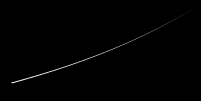
\includegraphics[width=0.38\textwidth]{example-mask.png}
  \caption{Example rendered image $R(x_t)$ for some hypothesis $x_t$.}
  \label{fig:example-mask}
\end{figure}

\section{Preprocessing of real images}
\label{prep-real}

In the images of real rodents used for testing, the rodent was
illuminated from below, meaning it and its whiskers were dark against
a bright background. The filtering function described in the previous
section expects whisker pixels to be bright and the body has the same 
pixel values as the whiskers, so the images had to be inverted.

\subsection{Subtracting background}
    Removing effects like difference in background illumination 
    and static objects is prefered to minimize faulty responses. 

    Assuming we always have a static camera setup foreach sequence and 
    that we have a adiquit sequence without the rodent.
    The background was captured a priori by taking a mean\ref{def:image_addition} 
    of the 100\footnote{Just a sufficient number} first frames $BG$ 
    \begin{equation}
        I_{BG} = \frac{\sum\limits_{bg\in BG}{I_{bg}}}{\#\left\{BG\right\}}.
    \end{equation}
    <<image showing the mean background>>

    Then we can simply subtract\ref{def:image_subtraction} the background $I_{BG}$ 
    from the orignal image $I$
    \footnote{
    Worth noting is that more sofisticated methods exists to subtract the background, 
    but this solution works relatively well considering the simplicity.
    }
   
    \begin{equation}
        I_{FG} = I - I_{BG}
    \end{equation}
    <<example with the 3 images involved above alongside eachother>>


\subsection{Finding the body $\prob{\text{body}}$}
    Finding the body has two purposes, firstly to find the head-coordinate system 
    and secondly to subtract the body from the image to find whiskers.
    \begin{definition}
        \begin{equation}
            \prob{\text{body}}\in \IS
        \end{equation} Is an estimation\footnote{Only needs to be an indication on wether 
        it is a body} on the probablity of the pixel to be a householding a rodent body.
    \end{definition}
    Assuming that the only non-static objects in the image is the whiskers and body.
    One simple feature that easily classifies $\prob{\text{whisker}}$ from 
    $\prob{\text{body}}$ is size. Bluring the image removes fine structures 
    and retains larger ones.
    This was performed by convoluting the image with a gaussian with ${\sigma=9}$px\footnote{The value for $\sigma$ was obtained by manual testing.}
    \begin{equation}
        \prob{\text{body}} = I_{blur} = I_{FG}\star \text{gauss}(0,\sigma)
    \end{equation}
    <<example of the blur showing that the whiskers has almost disapeared>>
    Which then was made to a mask by 
    \begin{equation}
        \text{body} = \prob{\text{body}}>0.6 \in \IS.\footnote{0.6 found to be a value making the body stable between frames}
    \end{equation}
    representing the location of the body.
    <<example showing p(body) och body alongside each other>>

\subsection{Estimating $\prob{whisker}$}
    Getting an indicator on the location of whiskers is needed for the filtering.\ref{sec:filtering}
    \begin{definition}
        \begin{equation}
            \prob{whisker}\in \IS
        \end{equation} Is an estimation\footnote{Only needs to be an indication on wether it is a whisker} on the probablity of the pixel to be a householding a rodent whisker.
    \end{definition}
    This is na\"{i}vly performed by
    \begin{equation}
        \prob{\text{whisker}} = I_{FG}*(1-\text{body})
    \end{equation}

    <<example showing the above>>

\subsection{Estimate snout translation}
    Firstly we hand pick the first frame where the snout is fully visible and use this frame as reference to estimate the translation.
    The mask is then again blured out with a $\sigma=$5px\footnote{Obtained by manual testing.} and filtered through a prewittfilter
    
    \begin{equation}
       \text{snout}_{ref} = \sqrt{(\text{snout} \star \text{prewitt}_x)^2 + ( \text{snout} \star \text{prewitt}_y )^2}\in\IS
    \end{equation}
    to smooth out the response of the edges.

    Then a local search within $5$px\footnote{This could easily be extended to include rotation.} from the last location was 
    performed foreach image in the sequence
    \begin{equation}
       \text{translation} = \argmax{(x,y)\in\text{close}}
                                {
                                    (\sum 
                                        \text{translate}(\text{snout}_{ref},-(x,y))*\text{snout}
                                    )
                                } \in \ZZ^2
    \end{equation}
    where $\text{snout}$ is the current image under the same filter as $\text{snout}_{ref}$

\subsection{Fixate the head programmatically}
    As a last touch we transform the video to fixate the head coordinates to 
    simplify the tracking analysis, 
    this will not effect the final result one could simply pass 
    the moving coordinate system directly to the tracker. 

